%%%%%%%%%%%%%%%%%%%%%%%%%%%%%%%%%%%%%%%%%%%%%%%%%%%%%%%%%%%%%%%%%%%%%%
%%  Copyright by Wenliang Du.                                       %%
%%  This work is licensed under the Creative Commons                %%
%%  Attribution-NonCommercial-ShareAlike 4.0 International License. %%
%%  To view a copy of this license, visit                           %%
%%  http://creativecommons.org/licenses/by-nc-sa/4.0/.              %%
%%%%%%%%%%%%%%%%%%%%%%%%%%%%%%%%%%%%%%%%%%%%%%%%%%%%%%%%%%%%%%%%%%%%%%

\newcommand{\commonfolder}{../../common-files}

\documentclass[11pt]{article}

\usepackage[most]{tcolorbox}
\usepackage{times}
\usepackage{epsf}
\usepackage{epsfig}
\usepackage{amsmath, alltt, amssymb, xspace}
\usepackage{wrapfig}
\usepackage{fancyhdr}
\usepackage{url}
\usepackage{verbatim}
\usepackage{fancyvrb}
\usepackage{adjustbox}
\usepackage{listings}
\usepackage{color}
\usepackage{subfigure}
\usepackage{cite}
\usepackage{sidecap}
\usepackage{pifont}
\usepackage{mdframed}
\usepackage{textcomp}
\usepackage{enumitem}


% Horizontal alignment
\topmargin      -0.50in  % distance to headers
\oddsidemargin  0.0in
\evensidemargin 0.0in
\textwidth      6.5in
\textheight     8.9in 

\newcommand{\todo}[1]{
\vspace{0.1in}
\fbox{\parbox{6in}{TODO: #1}}
\vspace{0.1in}
}


\newcommand{\unix}{{\tt Unix}\xspace}
\newcommand{\linux}{{\tt Linux}\xspace}
\newcommand{\minix}{{\tt Minix}\xspace}
\newcommand{\ubuntu}{{\tt Ubuntu}\xspace}
\newcommand{\setuid}{{\tt Set-UID}\xspace}
\newcommand{\openssl} {\texttt{openssl}}


\pagestyle{fancy}
\lhead{\bfseries SEED Labs}
\chead{}
\rhead{\small \thepage}
\lfoot{}
\cfoot{}
\rfoot{}


\definecolor{dkgreen}{rgb}{0,0.6,0}
\definecolor{gray}{rgb}{0.5,0.5,0.5}
\definecolor{mauve}{rgb}{0.58,0,0.82}
\definecolor{lightgray}{gray}{0.90}


\lstset{%
  frame=none,
  language=,
  backgroundcolor=\color{lightgray},
  aboveskip=3mm,
  belowskip=3mm,
  showstringspaces=false,
%  columns=flexible,
  basicstyle={\small\ttfamily},
  numbers=none,
  numberstyle=\tiny\color{gray},
  keywordstyle=\color{blue},
  commentstyle=\color{dkgreen},
  stringstyle=\color{mauve},
  breaklines=true,
  breakatwhitespace=true,
  tabsize=3,
  columns=fullflexible,
  keepspaces=true,
  escapeinside={(*@}{@*)}
}

\newcommand{\newnote}[1]{
\vspace{0.1in}
\noindent
\fbox{\parbox{1.0\textwidth}{\textbf{Note:} #1}}
%\vspace{0.1in}
}


%% Submission
\newcommand{\seedsubmission}{You need to submit a detailed lab report, with screenshots,
to describe what you have done and what you have observed.
You also need to provide explanation
to the observations that are interesting or surprising.
Please also list the important code snippets followed by
explanation. Simply attaching code without any explanation will not
receive credits.}

%% Book
\newcommand{\seedbook}{\textit{Computer \& Internet Security: A Hands-on Approach}, 2nd
Edition, by Wenliang Du. See details at \url{https://www.handsonsecurity.net}.}

%% Videos
\newcommand{\seedisvideo}{\textit{Internet Security: A Hands-on Approach},
by Wenliang Du. See details at \url{https://www.handsonsecurity.net/video.html}.}

\newcommand{\seedcsvideo}{\textit{Computer Security: A Hands-on Approach},
by Wenliang Du. See details at \url{https://www.handsonsecurity.net/video.html}.}

%% Lab Environment
\newcommand{\seedenvironment}{This lab has been tested on our pre-built
Ubuntu 16.04 VM, which can be downloaded from the SEED website. }

\newcommand{\seedenvironmentA}{This lab has been tested on our pre-built
Ubuntu 16.04 VM, which can be downloaded from the SEED website. }

\newcommand{\seedenvironmentB}{This lab has been tested on our pre-built
Ubuntu 20.04 VM, which can be downloaded from the SEED website. }

\newcommand{\seedenvironmentAB}{This lab has been tested on our pre-built
Ubuntu 16.04 and 20.04 VMs, which can be downloaded from the SEED website. }

\newcommand{\nodependency}{Since we use containers to set up the lab environment, 
this lab does not depend too much on our SEED VM. You can do this lab
using other VMs or physical machines. }







\newcommand{\seedlabcopyright}[1]{
\vspace{0.1in}
\fbox{\parbox{6in}{\small Copyright \copyright\ {#1}\ \ by Wenliang Du.\\
      This work is licensed under a Creative Commons
      Attribution-NonCommercial-ShareAlike 4.0 International License.
      If you remix, transform, or build upon the material, 
      this copyright notice must be left intact, or reproduced in a way that is reasonable to
      the medium in which the work is being re-published.}}
\vspace{0.1in}
}





\newcommand{\pcap} {\texttt{pcap}\xspace}
\newcommand{\telnet} {\texttt{telnet}\xspace}

\lhead{\bfseries SEED Labs -- Packet Sniffing and Spoofing Lab}


\begin{document}



\begin{center}
{\LARGE Packet Sniffing and Spoofing Lab}
\end{center}

\seedlabcopyright{2006 - 2020}


\newcounter{task}
\setcounter{task}{1}
\newcommand{\tasks} {\bf {\noindent (\arabic{task})} \addtocounter{task}{1} \,}

\section{Overview}

Packet sniffing and spoofing are two important concepts in
network security; they are two major threats in network 
communication. Being able to understand these two threats 
is essential for understanding security measures in 
networking. There are many packet sniffing and spoofing tools,
such as {\tt Wireshark}, {\tt Tcpdump}, {\tt Netwox}, \texttt{Scapy}, etc.
Some of these tools are widely used by security experts, as well as by
attackers. Being able to use these tools is important
for students, but what is more important for students in 
a network security course is to understand how these tools work,
i.e., how packet sniffing and spoofing are implemented  
in software.

The objective of this lab is two-fold: learning to use the tools 
and understanding the technologies underlying these tools. 
For the second object, students will write simple sniffer and spoofing programs,
and gain an in-depth understanding of the technical aspects of these programs.
This lab covers the following topics:


\begin{itemize}[noitemsep]
\item How the sniffing and spoofing work
\item Packet sniffing using the {\tt pcap} library and Scapy
\item Packet spoofing using raw socket and Scapy
\item Manipulating packets using Scapy 
\end{itemize}



\paragraph{Readings and Videos.}
Detailed coverage of sniffing and spoofing can be found in
the following:

\begin{itemize}
\item Chapter 15 of the SEED Book, \seedbook

\item Section 2 of the SEED Lecture, \seedisvideo
\end{itemize}



\paragraph{Lab environment.} \seedenvironment



\paragraph{Note for Instructors.}
There are two sets of tasks in this lab. The first set focuses on using 
tools to conduct packet sniffing and spoofing. It only requires a
little bit of Python programming (usually a few lines of code); students do
not need to have a prior Python programming background. 
The set of tasks can be used by students with a much broader background.

The second set of tasks is designed primarily for Computer Science/Engineering students.
Students need to write their own C programs from the scratch to do sniffing 
and spoofing. This way, they can gain a deeper understanding 
on how sniffing and spoofing tools actually work. Students 
need to have a solid programming background for these tasks.
The two sets of tasks are independent; instructors can choose to
assign one set or both sets to their students, depending on 
their students' programming background.


% *******************************************
% SECTION
% ******************************************* 
\section{Environment Setup using Container} 

In this lab, we will use two machines that are connected
to the same LAN. We can either use two VMs or use two containers. 
Figure~\ref{fig:labsetup} depicts the lab environment setup using 
containers.
We will do all the attacks on the attacker container, while using
the other container as the user machine. 


\begin{figure}[htb]
\begin{center}
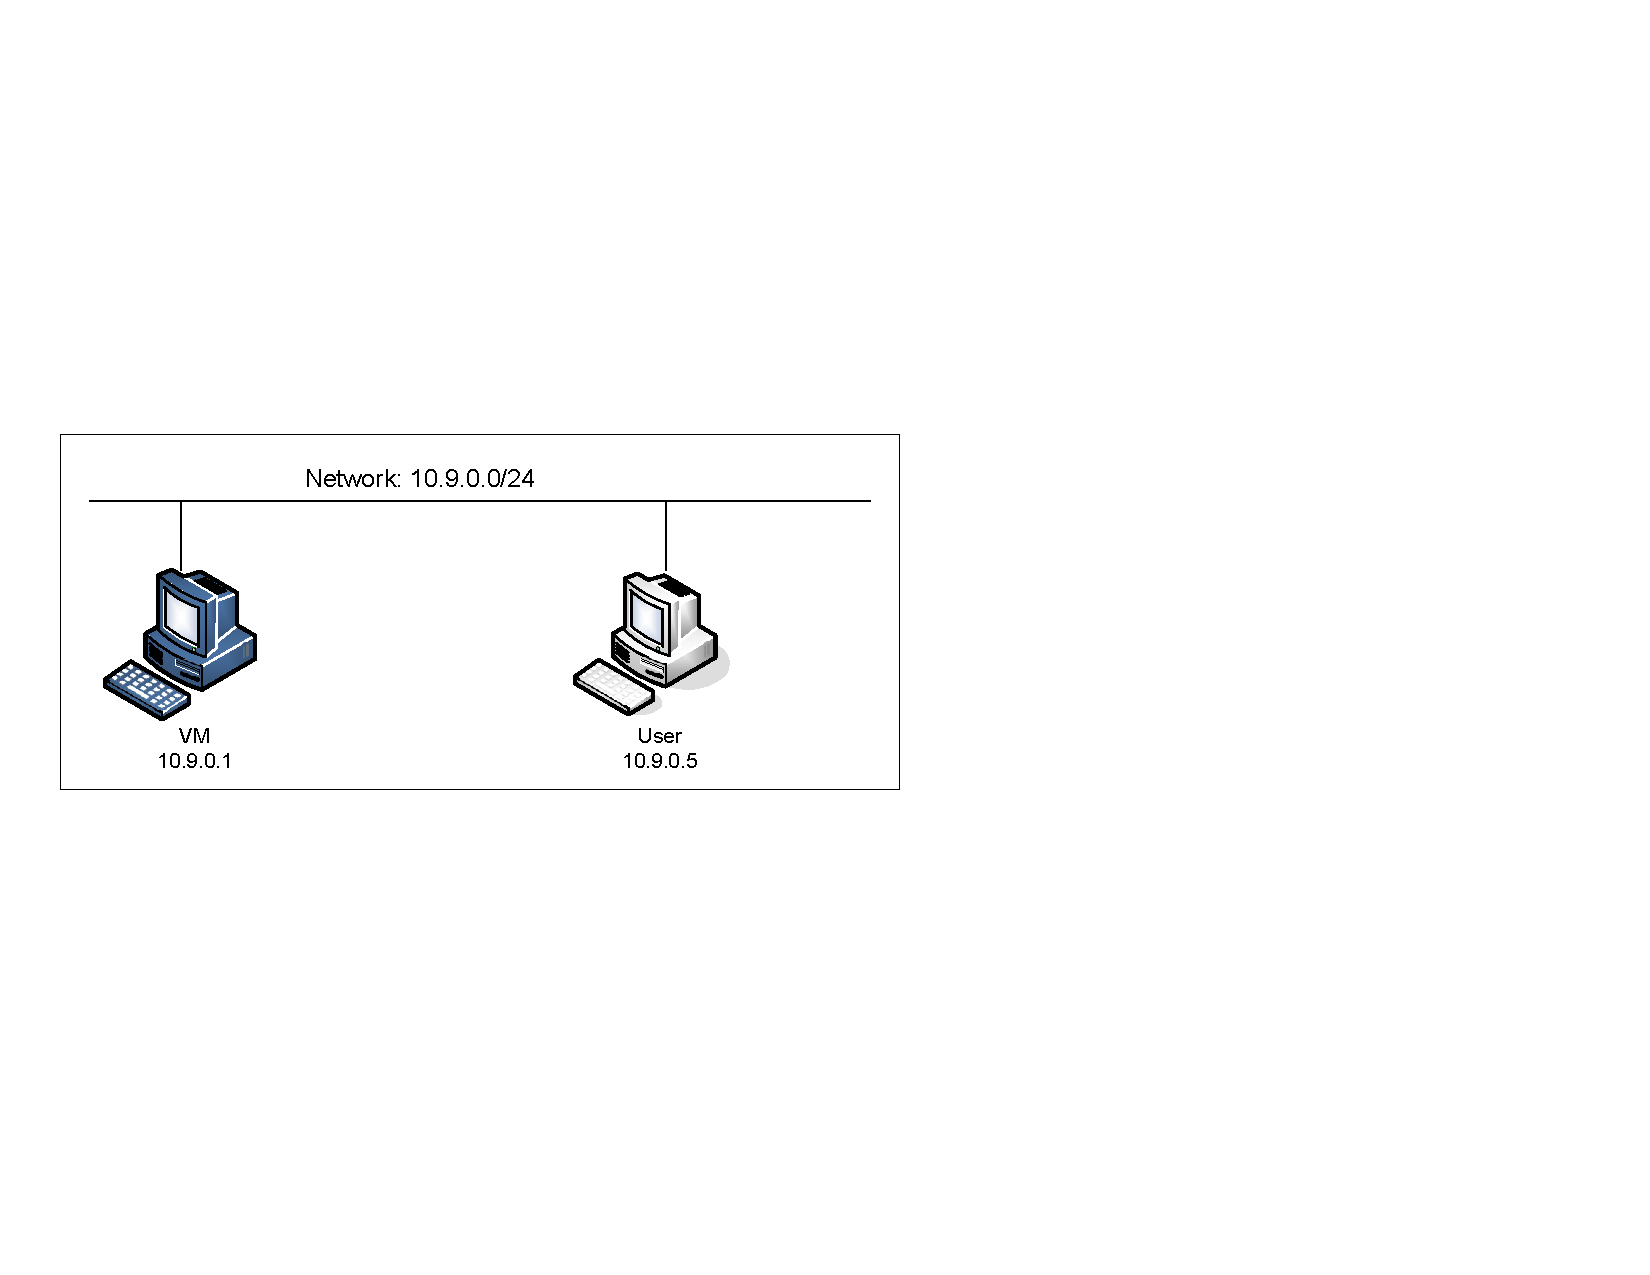
\includegraphics[width=0.8\textwidth]{\commonfolder/Figs/OneLan_onehost.pdf}
\end{center}
\caption{Lab environment setup}
\label{fig:labsetup}
\end{figure}
 

%\begin{lstlisting}[backgroundcolor=]
%                +--------------+      +--------------+
%                |  (attacker)  |      |    (user)    |
%                |   10.9.0.1   |      |   10.9.0.5   |
%                +-----+--------+      +------+-------+
%                      | br-<id>              | eth0
%         10.9.0.0/24  |                      |
%         -------------+----------------------+------------
%
%\end{lstlisting}
 


% -------------------------------------------
% SUBSECTION
% -------------------------------------------
\subsection{Container Setup and Commands} 

%%%%%%%%%%%%%%%%%%%%%%%%%%%%%%%%%%%%%%%%%%%%
Please download the
\texttt{Labsetup.zip} file to your VM from the lab's website,
unzip it, enter the \texttt{Labsetup} folder, and 
use the \texttt{docker-compose.yml} file to 
set up the lab environment. Detailed explanation
of the content in this file and all the involved 
\texttt{Dockerfile} can be found from the 
user manual, which is linked to the website of this lab.
If this is the first time you set up a SEED lab environment
using containers, it is very important that you read 
the user manual. 

In the following, we list some of the commonly
used commands related to Docker and Compose. 
Since we are going to use 
these commands very frequently, we have created aliases for them
in the \texttt{.bashrc} file (in our provided SEEDUbuntu 20.04 VM).


\begin{lstlisting}
$ docker-compose build  # Build the container image
$ docker-compose up     # Start the container
$ docker-compose down   # Shut down the container

// Aliases for the Compose commands above
$ dcbuild       # Alias for: docker-compose build
$ dcup          # Alias for: docker-compose up
$ dcdown        # Alias for: docker-compose down
\end{lstlisting}


All the containers will be running in the background. To run
commands on a container, we often need to get a shell on
that container. We first need to use the \texttt{"docker ps"}  
command to find out the ID of the container, and then
use \texttt{"docker exec"} to start a shell on that 
container. We have created aliases for them in
the \texttt{.bashrc} file.

\begin{lstlisting}
$ dockps        # Alias for: docker ps --format "{{.ID}}  {{.Names}}" 
$ docksh <id>   # Alias for: docker exec -it <id> /bin/bash

# The following example shows how to get a shell inside hostC
$ dockps
b1004832e275  hostA-10.9.0.5
0af4ea7a3e2e  hostB-10.9.0.6
9652715c8e0a  hostC-10.9.0.7

$ docksh 96
root@9652715c8e0a:/#  

# Note: If a docker command requires a container ID, you do not need to 
#       type the entire ID string. Typing the first few characters will 
#       be sufficient, as long as they are unique among all the containers. 
\end{lstlisting}


If you encounter problems when setting up the lab environment, 
please read the ``Common Problems'' section of the manual
for potential solutions.


%%%%%%%%%%%%%%%%%%%%%%%%%%%%%%%%%%%%%%%%%%%%


% -------------------------------------------
% SUBSECTION
% -------------------------------------------
\subsection{About the Attacker Container}

In this lab, we can either use the VM or the attacker container
as the attacker machine. If you look at the Docker Compose file, you will
see that the attacker container is configured differently from the other
containers. Here are the differences:


\begin{itemize}
\item \textit{Shared folder.} When we use the attacker container
to launch attacks, we need to put the attacking code inside
the attacker container.
%%%%%%%%%%%%%%%%%%%%%%%%%%%%%%%%%%%%%%%%%%%%%%%
Code editing is more convenient inside the VM than in a container, 
because we can use our favorite editor to write code. 
In order for the VM and a container to share files, 
we have created a shared folder between VM and the container
using the Docker \texttt{volumes}.
If you look at the Docker Compose file, you will find out that
we have added the following entry to some of the containers.
It indicates mounting the \texttt{./volumes} folder on the host
machine (i.e., the VM) to the \texttt{/volumes} folder inside the container.
We will write our code in the \texttt{./volumes} folder (on the VM), so they
can be used inside the containers.

\begin{lstlisting}
volumes:
       - ./volumes:/volumes
\end{lstlisting}


%%%%%%%%%%%%%%%%%%%%%%%%%%%%%%%%%%%%%%%%%%%%%%%


\item \textit{Host mode.}
%%%%%%%%%%%%%%%%%%%%%%%%%%%%%%%%%%%%%%%%%%%%%%%
In this lab, the attacker needs to be able to sniff packets,
but running sniffer programs inside a container has problems, because
a container is effectively attached to a virtual switch, 
so it can only see its own traffic, and it is never going to see 
the packets among other containers. To solve this problem,
we use the \texttt{host} mode for the attacker container. This
allows the attacker container to see all the traffics. The following
entry used on the attacker container:

\begin{lstlisting}
network_mode: host
\end{lstlisting}

When a container is in the \texttt{host} mode,  it sees
all the host's network interfaces, and it even has the same
IP addresses as the host. Basically, it is put in the
same network namespace as the host VM. However, the container
is still a separate machine, because its other namespaces are
still different from the host.


%%%%%%%%%%%%%%%%%%%%%%%%%%%%%%%%%%%%%%%%%%%%%%%
\end{itemize}


\paragraph{Getting the network interface name.}
%%%%%%%%%%%%%%%%%%%%%%%%%%%%%%%%%%%%%%%%%%%%%%%

\paragraph{Getting the network interface name.}
When we use the provided Compose file to create
containers for this lab, a new network is created
to connect the VM and the containers. The
IP prefix for this network is \texttt{10.9.0.0/24},
which is specified in the \texttt{docker-compose.yml}
file. The IP address assigned to our VM is
\texttt{10.9.0.1}. We need to find the name of
the corresponding network interface on our VM, because we
need to use it in our programs.
The interface name is the concatenation of \texttt{br-}
and the ID of the network created by Docker.
When we use \texttt{ifconfig} to list network interfaces,
we will see quite a few. Look for the IP address
\texttt{10.9.0.1}.


\begin{lstlisting}
$ ifconfig
(*@\textbf{br-c93733e9f913}@*): flags=4163<UP,BROADCAST,RUNNING,MULTICAST>  mtu 1500
        inet (*@\textbf{10.9.0.1}@*)  netmask 255.255.255.0  broadcast 10.9.0.255
        ...
\end{lstlisting}


Another way to get the interface name is to use the \texttt{"docker network"} command to
find out the network ID ourselves (the name of the network is \texttt{seed-net}:

\begin{lstlisting}
$ docker network ls
NETWORK ID          NAME                DRIVER              SCOPE
a82477ae4e6b        bridge              bridge              local
e99b370eb525        host                host                local
df62c6635eae        none                null                local
(*@\textbf{c93733e9f913}@*)        seed-net            bridge              local
\end{lstlisting}



%%%%%%%%%%%%%%%%%%%%%%%%%%%%%%%%%%%%%%%%%%%%%%%



% *******************************************
% SECTION
% ******************************************* 
\section{Lab Task Set 1: Using Tools to Sniff and Spoof Packets}


Many tools can be used to do sniffing and spoofing, but most of them only provide 
fixed functionalities. Scapy is different: it can be used not only as a tool, 
but also as a building block to construct other sniffing and spoofing
tools, i.e., we can integrate the Scapy functionalities into our own
program.  In this set of tasks, we will use Scapy for each task. 


To use Scapy, we can write a Python program, and then execute this program
using Python. See the following example. We should run Python using the 
root privilege because the privilege is required for spoofing packets. 
At the beginning of the program (Line~\ding{192}), 
we should import all Scapy's modules.

\begin{lstlisting}
# view mycode.py
#!/usr/bin/env python3

from scapy.all import *    (*@\ding{192}@*)

a = IP()
a.show()

# python3 mycode.py
###[ IP ]###
  version   = 4
  ihl       = None
  ...


// Make mycode.py executable (another way to run python programs)
# chmod a+x mycode.py
# mycode.py 
\end{lstlisting}


We can also get into the interactive mode of Python and
then run our program one line at a time at the Python prompt. 
This is more convenient if we need to change our code 
frequently in an experiment.

\begin{lstlisting}
# python3
>>> from scapy.all import *
>>> a = IP()
>>> a.show()
###[ IP ]###
  version   = 4
  ihl       = None
  ...
\end{lstlisting}
 

% -------------------------------------------
% SUBSECTION
% ------------------------------------------- 
\subsection{Task 1.1: Sniffing Packets}  


Wireshark is the most popular sniffing tool, and it is easy to use. We will use it throughout 
the entire lab. However, it is difficult to use Wireshark as a building block 
to construct other tools. We will use Scapy for that purpose. The objective of this task is to
learn how to use Scapy to do packet sniffing in Python programs. 
A sample code is provided in the following:


\begin{lstlisting}
#!/usr/bin/env python3
from scapy.all import *

def print_pkt(pkt):
  pkt.show()

pkt = sniff(iface='br-c93733e9f913', filter='icmp', prn=spoof_pkt)
\end{lstlisting}


The code above will sniff the packets on the \texttt{br-c93733e9f913}
interface. Please read the instruction in the lab setup section
regarding how to get the interface name. 
If we want to sniff on multiple interfaces, we can
put all the interfaces in a list, and assign it to \texttt{iface}.
See the following example: 


\begin{lstlisting}
iface=['br-c93733e9f913', 'enp0s3']
\end{lstlisting}
 


\paragraph{Task 1.1A.} The above program sniffs packets. For each captured
packet, the callback function \texttt{print\_pkt()} will be invoked; this function will print out some of
the information about the packet. Run the program with the root privilege and demonstrate that
you can indeed capture packets. After that, run the program again, but without using the root
privilege; describe and explain your observations. 
 
\begin{lstlisting}
// Make the program executable 
# chmod a+x sniffer.py

// Run the program with the root privilege
# sniffer.py

// Switch to the "seed" account, and
// run the program without the root privilege
# su seed
$ sniffer.py
\end{lstlisting}


\paragraph{Task 1.1B.} Usually, when we sniff packets, we are only
interested certain types of packets. We can do that by setting 
filters in sniffing. Scapy's filter use the 
BPF (Berkeley Packet Filter) syntax; you can find the BPF manual 
from the Internet. Please set the following filters and demonstrate 
your sniffer program again (each filter should be set separately):

\begin{itemize} 
 \item Capture only the ICMP packet
 \item Capture any TCP packet that comes from a particular IP and with 
 a destination port number 23. 
 \item Capture packets comes from or to go to a particular subnet. You can
 pick any subnet, such as \texttt{128.230.0.0/16}; you should not 
 pick the subnet that your VM is attached to. 
\end{itemize} 



% -------------------------------------------
% SUBSECTION
% ------------------------------------------- 
\subsection{Task 1.2: Spoofing ICMP Packets}

As a packet spoofing tool, Scapy allows us to set the fields of 
IP packets to arbitrary values. The objective of this 
task is to spoof IP packets with an arbitrary source IP address. 
We will spoof ICMP echo request packets, and send them to another VM on
the same network. We will use Wireshark to observe
whether our request will be accepted by the receiver. If it is accepted, an
echo reply packet will be sent to the spoofed IP address. 
The following code shows an example of how to spoof an ICMP packets.


\begin{lstlisting}
>>> from scapy.all import *
>>> a = IP()              (*@\ding{192}@*)
>>> a.dst = '10.0.2.3'    (*@\ding{193}@*)
>>> b = ICMP()            (*@\ding{194}@*)
>>> p = a/b               (*@\ding{195}@*)
>>> send(p)               (*@\ding{196}@*)
.
Sent 1 packets.
\end{lstlisting}
 

In the code above, Line~\ding{192} creates an IP object from the IP class; 
a class attribute is defined for each IP header field. We
can use \texttt{ls(a)} or \texttt{ls(IP)} to see all 
the attribute names/values. We can also use a.show() and IP.show() to do
the same. Line~\ding{193} shows how to set the destination 
IP address field. If a field is not set, a default value will be 
used. 

\begin{lstlisting}
>>> ls(a)
version    : BitField (4 bits)       = 4               (4)
ihl        : BitField (4 bits)       = None            (None)
tos        : XByteField              = 0               (0)
len        : ShortField              = None            (None)
id         : ShortField              = 1               (1)
flags      : FlagsField (3 bits)     = <Flag 0 ()>     (<Flag 0 ()>)
frag       : BitField (13 bits)      = 0               (0)
ttl        : ByteField               = 64              (64)
proto      : ByteEnumField           = 0               (0)
chksum     : XShortField             = None            (None)
src        : SourceIPField           = '127.0.0.1'     (None)
dst        : DestIPField             = '127.0.0.1'     (None)
options    : PacketListField         = []              ([])
\end{lstlisting}
 

Line~\ding{194} creates an ICMP object. The default type is echo request.
In Line~\ding{195}, we stack \texttt{a} and \texttt{b} together to 
form a new object. The \texttt{/} operator is overloaded by the
IP class, so it no longer represents division; instead, it means 
adding \texttt{b} as the payload field of \texttt{a} and modifying
the fields of \texttt{a} accordingly. As a result, we get a new 
object that represent an ICMP packet. We can now send out this packet 
using \texttt{send()} in Line~\ding{196}. Please make any necessary change
to the sample code, and then demonstrate that you can spoof an ICMP echo
request packet with an arbitrary source IP address. 



% -------------------------------------------
% SUBSECTION
% ------------------------------------------- 
\subsection{Task 1.3: Traceroute} 

The objective of this task is to use Scapy to estimate the distance, in
terms of number of routers, between your VM and a selected destination.  
This is basically what is implemented by the \texttt{traceroute} tool. 
In this task, we will write our own tool. The idea is quite
straightforward: just send an packet (any type) to the destination, with
its Time-To-Live (TTL) field set to 1 first. This packet will be dropped by
the first router, which will send us an ICMP error message, telling us 
that the time-to-live has exceeded. That is how we get the IP address of
the first router. We then increase our TTL field to 2, send out another
packet, and get the IP address of the second router. We will repeat this
procedure until our packet finally reach the destination. It should be
noted that this experiment only gets an estimated result, because in
theory, not all these packets take the same route (but in practice, they may
within a short period of time). The code in the following shows one round 
in the procedure. 


\begin{lstlisting}
a = IP()
a.dst = '1.2.3.4'
a.ttl = 3
b = ICMP()
send(a/b)
\end{lstlisting}


If you are an experienced Python programmer, you can write your tool 
to perform the entire procedure automatically. If you are new to Python
programming, you can do it by manually changing the TTL field in 
each round, and record the IP address based on your observation 
from Wireshark. Either way is acceptable, as long as you get the result. 


% -------------------------------------------
% SUBSECTION
% ------------------------------------------- 
\subsection{Task 1.4: Sniffing and-then Spoofing}  

In this task, you will combine the sniffing and spoofing techniques
to implement the following sniff-and-then-spoof program.
You need two machines on the same LAN: the VM and the user container. 
From the user container, you
{\tt ping} an IP X. This will generate an ICMP echo
request packet. If X is alive, the {\tt ping} program will receive
an echo reply, and print out the response. Your sniff-and-then-spoof
program runs on the VM, which monitors the LAN through packet sniffing. Whenever it
sees an ICMP echo request, regardless of what the target IP address is,
your program should immediately send out an echo reply using the
packet spoofing technique. Therefore, regardless of whether machine X
is alive or not, the {\tt ping} program will always receive
a reply, indicating that X is alive. You need to use Scapy
to do this task. In your report, you need to provide evidence to demonstrate 
that your technique works. 

In your experiment, you should \texttt{ping} the following three IP addresses
from the user container. 
Report your observation and explain the results. 

\begin{lstlisting}
ping 1.2.3.4     # a non-existing host on the Internet
ping 10.9.0.99   # a non-existing host on the LAN
ping 8.8.8.8     # an existing host on the Internet
\end{lstlisting}

\paragraph{Hint:} You need to understand how the ARP protocol works in order to 
correctly explain your observation. You also need to know a little bit 
about routing. The following command help you find the router
for a specified destination:

\begin{lstlisting}
ip route get 1.2.3.4 
\end{lstlisting}
 
 


% *******************************************
% SECTION
% ******************************************* 
\section{Lab Task Set 2: Writing Programs to Sniff and Spoof Packets}



% -------------------------------------------
% SUBSECTION
% ------------------------------------------- 
\subsection{Task 2.1: Writing Packet Sniffing Program}

Sniffer programs can be easily written using the \pcap library. With \pcap, 
the task of 
sniffers becomes invoking a simple sequence of procedures
in the \pcap library. At the end of the sequence,
packets will be put in buffer for further processing
as soon as they are captured. All the details 
of packet capturing are handled by the \pcap library.


The SEED book ``\textit{Computer Security: A Hands-on Approach}'' provides a sample code 
in Chapter 12, showing how  to write a simple sniffer program using 
\pcap. We include the sample code in the following (see the book for detailed explanation). 

\begin{lstlisting}
#include <pcap.h>
#include <stdio.h>

/* This function will be invoked by pcap for each captured packet.
   We can process each packet inside the function.  
 */
void got_packet(u_char *args, const struct pcap_pkthdr *header,
        const u_char *packet)
{
   printf("Got a packet\n");
}

int main()
{
  pcap_t *handle;
  char errbuf[PCAP_ERRBUF_SIZE];
  struct bpf_program fp;
  char filter_exp[] = "ip proto icmp";
  bpf_u_int32 net;

  // Step 1: Open live pcap session on NIC with name eth3
  //         Students needs to change "eth3" to the name 
  //         found on their own machines (using ifconfig).
  handle = pcap_open_live("eth3", BUFSIZ, 1, 1000, errbuf); 

  // Step 2: Compile filter_exp into BPF psuedo-code
  pcap_compile(handle, &fp, filter_exp, 0, net);            
  pcap_setfilter(handle, &fp);                              

  // Step 3: Capture packets
  pcap_loop(handle, -1, got_packet, NULL);                  

  pcap_close(handle);   //Close the handle
  return 0;
}

// Note: don't forget to add "-lpcap" to the compilation command.
// For example: gcc -o sniff sniff.c -lpcap
\end{lstlisting}


Tim Carstens has also written a tutorial on how to use 
\pcap library to write a sniffer program. The tutorial is 
available at \url{http://www.tcpdump.org/pcap.htm}.  
 

\paragraph{Task 2.1A: Understanding How a Sniffer Works}
In this task, students need to write a sniffer program to 
print out the source and destination IP addresses of each captured 
packet. Students can type in the above code or download the sample code from the 
SEED book's website (\url{https://www.handsonsecurity.net/figurecode.html}). 
Students should provide screenshots as evidences to show that their sniffer
program can run successfully and produces expected 
results. In addition, please answer the following questions:

\begin{itemize}
\item \textbf{Question 1.} Please use your own words to describe the sequence of the 
library calls that are essential for sniffer programs. This 
is meant to be a summary, not detailed explanation like the 
one in the tutorial or book.
 
\item \textbf{Question 2.} Why do you need the root privilege to run a sniffer program? Where
does the program fail if it is executed without the root privilege?


\item \textbf{Quesiton 3.} Please turn on and turn off the promiscuous mode in your sniffer
program. Can you demonstrate the difference when this mode is on and off? Please describe how
you can demonstrate this.
\end{itemize}


\paragraph{Task 2.1B: Writing Filters.}
Please write filter expressions for your sniffer program 
to capture each of the followings. You can find online 
manuals for \pcap filters.
In your lab reports, you need to include screenshots to show
the results after applying each of these filters. 
\begin{itemize}
\item Capture the ICMP packets between two specific hosts.
\item Capture the TCP packets with a destination port number 
      in the range from 10 to 100.  
\end{itemize}



\paragraph{Task 2.1C: Sniffing Passwords.}
Please show how you can use your sniffer program to capture the 
password when somebody is using \telnet on the 
network that you are monitoring. You may need to modify
your sniffer code to print out the data part of a captured TCP 
packet (\telnet uses TCP). It is acceptable if you print out the entire data part, and then
manually mark where the password (or part of it) is.




% -------------------------------------------
% SUBSECTION
% ------------------------------------------- 
\subsection{Task 2.2: Spoofing}

When a normal user sends out a packet, operating systems
usually do not allow the user to set all the fields in the protocol 
headers (such as TCP, UDP, and IP headers). OSes will
set most of the fields, while only allowing users to 
set a few fields, such as the destination IP address, 
the destination port number, etc.  However, if 
users have the root privilege, they can set any 
arbitrary field in the packet headers. This is 
called packet spoofing, and it can be done through
{\em raw sockets}. 


Raw sockets give programmers the absolute control over the packet 
construction, allowing programmers to construct any arbitrary packet, including 
setting the header fields and the payload. Using raw sockets is 
quite straightforward; it involves four steps: (1) create a raw socket,
(2) set socket option, (3) construct the packet, and (4) send 
out the packet through the raw socket. There are 
many online tutorials that can teach you how to 
use raw sockets in C programming. We have linked some tutorials
to the lab's web page. Please read them, and learn how to 
write a packet spoofing program. We show a simple skeleton of 
such a program. 


\begin{lstlisting}
int sd;
struct sockaddr_in sin;
char buffer[1024]; // You can change the buffer size

/* Create a raw socket with IP protocol. The IPPROTO_RAW parameter
 * tells the sytem that the IP header is already included;
 * this prevents the OS from adding another IP header.  */
sd = socket(AF_INET, SOCK_RAW, IPPROTO_RAW);
if(sd < 0) {
    perror("socket() error"); exit(-1);
}

/* This data structure is needed when sending the packets 
 * using sockets. Normally, we need to fill out several 
 * fields, but for raw sockets, we only need to fill out
 * this one field */
sin.sin_family = AF_INET;

// Here you can construct the IP packet using buffer[]  
//    - construct the IP header ...
//    - construct the TCP/UDP/ICMP header ...
//    - fill in the data part if needed ...
// Note: you should pay attention to the network/host byte order.


/* Send out the IP packet. 
 * ip_len is the actual size of the packet. */  
if(sendto(sd, buffer, ip_len, 0, (struct sockaddr *)&sin, 
              sizeof(sin)) < 0) {
      perror("sendto() error"); exit(-1);
}
\end{lstlisting}



\paragraph{Task 2.2A: Write a spoofing program.}
Please write your own packet spoofing program in C. You need 
to provide evidences (e.g., Wireshark packet trace) to show that your 
program successfully sends out spoofed IP packets.


\paragraph{Task 2.2B: Spoof an ICMP Echo Request.}
Spoof an ICMP echo request packet on behalf of another machine (i.e., 
using another machine's IP address as its source IP address). This packet 
should be sent to a remote machine on the Internet (the machine must be
alive). You should turn on your Wireshark, so if your spoofing is successful, 
you can see the echo reply coming back from the remote machine. 



\paragraph{Questions.} Please answer the following questions.

\begin{itemize}
\item \textbf{Question 4.}
Can you set the IP packet length field to an arbitrary value,
regardless of how big the actual packet is? 


\item \textbf{Question 5.} 
Using the raw socket programming, do you have to calculate the 
checksum for the IP header? 

\item \textbf{Question 6.} 
Why do you need the root privilege to run the programs that 
use raw sockets? Where does the program fail if executed without the root 
privilege?

\end{itemize}
 





% -------------------------------------------
% SUBSECTION
% ------------------------------------------- 
\subsection{Task 2.3: Sniff and then Spoof}

In this task, you will combine the sniffing and spoofing techniques
to implement the following sniff-and-then-spoof program. 
You need two VMs on the same LAN. From VM A, you 
{\tt ping} an IP X. This will generate an ICMP echo 
request packet. If X is alive, the {\tt ping} program will receive 
an echo reply, and print out the response. Your sniff-and-then-spoof
program runs on VM B, which monitors the LAN through packet sniffing. Whenever it 
sees an ICMP echo request, regardless of what the target IP address is,
your program should immediately send out an echo reply using the 
packet spoofing technique. Therefore, regardless of whether machine X
is alive or not, the {\tt ping} program will always receive 
a reply, indicating that X is alive. You need to write such a program in C, and
include screenshots in your report to show that 
your program works. Please also attach the code (with adequate amount 
of comments) in your report.







% *******************************************
% SECTION
% ******************************************* 
\section{Guidelines} 



% -------------------------------------------
% SUBSECTION
% ------------------------------------------- 
\subsection{Filling in Data in Raw Packets}


When you send out a packet using raw sockets, you basically construct 
the packet inside a buffer, so when you need to send it out, you simply
give the operating system the buffer and the size of the packet. 
Working directly on the buffer is not easy, so a common way is to
typecast the buffer (or part of the buffer) into 
structures, such as IP header structure, so you can refer to the elements
of the buffer using the fields of those structures. 
You can define the IP, ICMP, TCP, UDP and other header structures in your 
program. The following example show how you can construct an UDP packet:

 
\begin{lstlisting}
struct ipheader {
   type  field;
   .....
}

struct udpheader {
   type field;
   ......
}

// This buffer will be used to construct raw packet.
char buffer[1024];

// Typecasting the buffer to the IP header structure
struct ipheader *ip = (struct ipheader *) buffer;

// Typecasting the buffer to the UDP header structure
struct udpheader *udp = (struct udpheader *) (buffer
                             + sizeof(struct ipheader));

// Assign value to the IP and UDP header fields.
ip->field = ...;
udp->field = ...;
\end{lstlisting}



% -------------------------------------------
% SUBSECTION
% ------------------------------------------- 
\subsection{Network/Host Byte Order and the Conversions}


You need to pay attention to the network and host byte orders. If you use 
x86 CPU, your host byte order uses {\em Little Endian}, while 
the network byte order uses {\em Big Endian}. Whatever the data you put 
into the packet buffer has to use the network byte order; if you do not 
do that, your packet will not be correct. You actually do not need to worry
about what kind of Endian your machine is using, and you actually should not worry
about if you want your program to be portable. 


What you need to do is to always remember to convert your data to the
network byte order when you place the data into the buffer, and convert
them to the host byte order when you copy the data from the buffer to 
a data structure on your computer. If the data is a single byte, you do not
need to worry about the order, but if the data is a {\tt short}, 
{\tt int}, {\tt long}, or a data type that consists of more than one byte, 
you need to call one of the following functions to convert the data:

\begin{lstlisting}
htonl(): convert unsigned int from host to network byte order.
ntohl(): reverse of htonl().
htons(): convert unsigned short int from host to network byte order.
ntohs(): reverse of htons().
\end{lstlisting}


You may also need to use {\tt inet\_addr()}, {\tt inet\_network()},
{\tt inet\_ntoa()}, {\tt inet\_aton()} to convert 
IP addresses from the dotted decimal form (a string) to a
32-bit integer of network/host byte order. You can get their 
manuals from the Internet.


 

% *******************************************
% SECTION
% ******************************************* 
\section{Submission}

%%%%%%%%%%%%%%%%%%%%%%%%%%%%%%%%%%%%%%%%

You need to submit a detailed lab report, with screenshots,
to describe what you have done and what you have observed.
You also need to provide explanation
to the observations that are interesting or surprising.
Please also list the important code snippets followed by
explanation. Simply attaching code without any explanation will not
receive credits.

%%%%%%%%%%%%%%%%%%%%%%%%%%%%%%%%%%%%%%%%



\end{document}


